\documentclass{article} %article 文档
\usepackage{anyfontsize} %设置字体大小
\usepackage{ctex}  %使用宏包(为了能够显示汉字)
\usepackage {amsmath} %数学公式
\setlength {\parindent} {0in} %段落缩进
\usepackage{graphicx}
\usepackage{float}
\usepackage{epstopdf}

\title{通过多模光纤同时传输射频和基带信号}  %文章标题
\author{Nishant Bindal·Rajanbir Singh Ghumaan·Prateek Jeet Singh Sohi·
 \\Nikhil Sharma·Hemdutt Joshi·Bharat Garg}%作者的名称
\date{Received:2 January 2021/Revised:23 February 2022/Accepted:9 March 2022
\\Published online:9 April 2022}       %日期

% 设置页面的环境,a4纸张大小,左右上下边距信息
\usepackage[a4paper,left=10mm,right=10mm,top=15mm,bottom=15mm]{geometry}  
\begin{document}

\maketitle          %添加这一句才能够显示标题等信息

\textbf{摘要}

数字图像处理是数字信号处理的一个子类别,重点是研究用于增强或恢复的处理技术。被各种类型的噪声破坏的图像
的去噪就属于这个类别。去噪主要是为了提高受影响图像的可理解性。用故障设备拍摄的图像或经过长途传输的图像
极易受到脉冲噪声的破坏,因此,提出了各种技术来去除图像中的这种噪声。每种技术都有自己的优点和缺点。本文
对这些技术进行了全面的比较分析,在广泛的噪声范围内进行了分析。所有的过滤技术都在MATLAB中实现,并用标准
的基准图像数据进行模拟,并对定性指标即峰值信噪比(PSNR)和结构相似度指数(SSIM)进行评估和比较。因此,
本文对各种最先进的噪声去除技术进行了全面的比较分析。
\bigskip

\textbf{关键词}
\quad 中位数滤波器,均值滤波器,盐和胡椒噪声,脉冲噪声,脉冲噪声,图像修复和去噪

\section{简介}
图像的失真可能会因噪声的干扰而导致有用的特征丢失。图像中的噪声可能源于图像捕获设备的缺陷、处理技术的失误、
传输到远距离时的干扰等因素。若要从视觉上分辨图像中是否存在脉冲噪声,观察者应寻找异常明亮或暗的像素。这些亮
或暗的像素对应着像素的最大值(255)或最小值(0)(对于8位图像,0和255是可能的最小和最大值)。利用各种图像
处理技术去除这些噪声的过程通常被称为去噪。\par

\hspace{2em}随着时间的推移,人们提出了各种用于恢复被盐和胡椒噪声破坏的图像的最先进的去噪滤波器。这篇
评论文章的主要目的是让读者了解各种不同的过滤器,以及这些过滤器可以被归类的各种类别的知识。这些论文的主要
贡献如下。

\begin{itemize}
\item 我们总结了大多数最先进的过滤器的工作技术。
\item 为了让读者更好地理解,还给出了使用各种技术过滤的选定基准图像(这些图像被密度为95 \% 的盐和胡椒噪声所破坏)的视觉表现。
\item 总而言之,本文将成为一个指南,使研究人员了解从1995年到2021年这四分之一世纪里盐和胡椒噪声去除领域的主要发展。
\end{itemize}

\hspace{2em}本文的其余部分组织如下。第3节解释了盐和胡椒噪声、其影响和不同的过滤技术。第4节向读者介绍了仿真
环境和对选定的过滤算法进行的比较分析。本节使用不同的表格和图表向读者介绍了这些过滤器在广泛的噪声密度范围内的
比较分析,即低度(不超过30\% )、中度(在30\%和90\%之间)和高度(超过90\%)。最后,在第5节中向读者提供了从
第4节得出的结论。

\section{评估参数}
对于各种过滤器的质量分析,使用了不同的质量评估指标。大体上,这些质量评估可以是主观的或定量的。主观的质量分析
是基于人眼从给定图像中提取结构信息的能力。然而,定量质量指标利用数学表达式来计算一个给定图像的质量。数学类很
容易实现,并提供统一的预测质量度量。在这种方法中,数学公式被应用于计算噪声/去噪声图像在原始图像上的噪声量。
在本文中,以下指标被用于质量分析。

\subsection{平均平方误差(MSE)}
平均平方误差或平均平方偏差(MSD)是处理后的像素值与准确的像素值之间的平均平方差。MSE的数学表达式由(1)给出。
\begin{equation}
    MSE= \frac{1}{M+N}\sum_{i=1}^M\sum_{i\j=1}^N(x_{i,j}-y_{i,j})^2
\end{equation}

\subsection{均方根误差(RMSE)}
RMSE可以计算为实际像素值和恢复后的像素值之间的平均平方差的根。它也可以通过取MSE的平方根来计算。
\begin{equation}
    RMSE=\sqrt{\frac{1}{M+N}\sum_{i=1}^M\sum_{i\j=1}^N(x_{i,j}-y_{i,j})^2}
\end{equation}

\subsection{峰值信噪比(PSNR)}
PSNR只是最大可能的信号功率与改变图像定量表示的噪声信号功率之间的比率。PSNR经常被用来衡量一项技术的修复精度。
PSNR可以被认为是人类对重建质量的一种近似感知。PSNR的数学表达式为分贝(dB),由(3)给出。
\begin{equation}
    PSNR=10\log_{10}({MAX^2}/{MSE})
\end{equation}
其中,MSE和MAX分别为信号的均方误差和最大值。

\subsection{结构相似性指数(SSIM)}
顾名思义,SSIM是用来测量修复/处理后的图像和实际图像之间的结构相似性。SSIM是以原始/未压缩的图像作为参考,对图
像质量进行的测量。
\begin{equation}
    SSIM=\frac{(2\mu_x\mu_y+C_1)(2\sigma_{xy}+C_2)}{(\mu_x^2+\mu_y^2+C_1)(\sigma_x^2+\sigma_y^2+C_2)}
\end{equation}
其中$\mu_x$($\sigma_x$)和$\mu_y$($\sigma_y$)分别是x和y方向的平均值(标准差)。而常数C1和C2的选择是为了使SSIM的最大(最小)值为1(0)。

\subsection{图像增强系数(IEF)}
IEF是实际图像和损坏图像的MSE与实际图像和重建图像的MSE之比,如(5)所示。它是估计去噪后图像质量提高的准确措施。
\begin{equation}
    IEF=\frac{\sum_{i=1}^M\sum_{j=1}^N(\hat{y}_{i,j}-x_{i,j})^2}{\sum_{i=1}^M\sum_{j=1}^N(y_{i,j}-x_{i,j})^2}
\end{equation}
(3)至(5)中使用的术语:M, N -图像的维度\par
\hspace{2em}$x_{i,j}$ -没有任何形式的噪声的实际图像\par
\hspace{2em}$y_{i,j}$ -去除噪音的图像\par
\hspace{2em}$\hat{y}_{i,j}$ -损坏的图像\par
\hspace{2em}MAX -函数给出图像的最大允许像素值。\par
\hspace{2em}本文主要围绕脉冲噪声及其去噪方法展开。脉冲噪声也可称为数据下降噪声,因为它在统计上将像素值的强度
下降到最大或最小的可能值。因此,也被称为 "盐和胡椒噪声"。本文试图解决许多研究人员在脉冲噪声去除技术方面的著名
技术。

\section{不同的盐和胡椒的噪音消除器}
\subsection{前提概念}
术语 "窗口 "或 "内核 "指的是预定大小的像素的邻域。通常情况下,在过滤过程中采取三种窗口尺寸。3×3、5×5和7×7。
在去噪过程中,考虑到较高的窗口尺寸,噪声效应会减少,但图像会失去其特征。在低噪声密度下,小的处理窗口可以有更
好的性能。在高噪声密度下,大的窗口尺寸会有更好的结果,但会增加图像的模糊效果。

\hspace{2em}滤波是一种增强图像的技术。在这种技术中,恢复的图像中的像素是通过对噪声及其邻近的像素进行一些操作
来计算的。在图像过滤中,有一些操作被应用,如平滑、锐化和边缘增强。滤波技术可以在空间域或频率域进行。在空间域中,
这些操作直接应用于图像的像素上。另一方面,在频域中,滤波操作是通过使用傅里叶变换或任何其他图像函数的变换将空间
域映射到频域来进行的。然而,本文介绍了各种最先进的空间滤波技术,如图1所示。用于消除盐和胡椒噪声的各种滤波技术分
为以下几类。

\subsection{线性滤波器}
在这些过滤技术中,恢复的像素被计算为以噪声像素为中心的特定大小的窗口的像素值的线性组合。这些技术通常伴随着模糊
效应,并且在去除诸如信号相关噪声方面表现不佳。最常见的线性滤波器是下面讨论的平均数或平均滤波器。

\subsubsection{均值滤波器}
平均值过滤器是最简单的过滤器之一。它是一个基于平均老化技术的线性滤波器。处理窗口通常是一个正方形的形状。这个
滤波器计算中心噪声像素周围的处理窗口的平均值,中心像素的值被计算的值所取代。损坏图像的平均值在Sxy定义的区域
内计算[1, 5, 6, 24]。
\begin{equation}
    f(x,y)=\frac{1}{MN}\sum_{(s,t)\in S_{xy}}g(s,t)
\end{equation}
\begin{figure}[H]
    \centering
    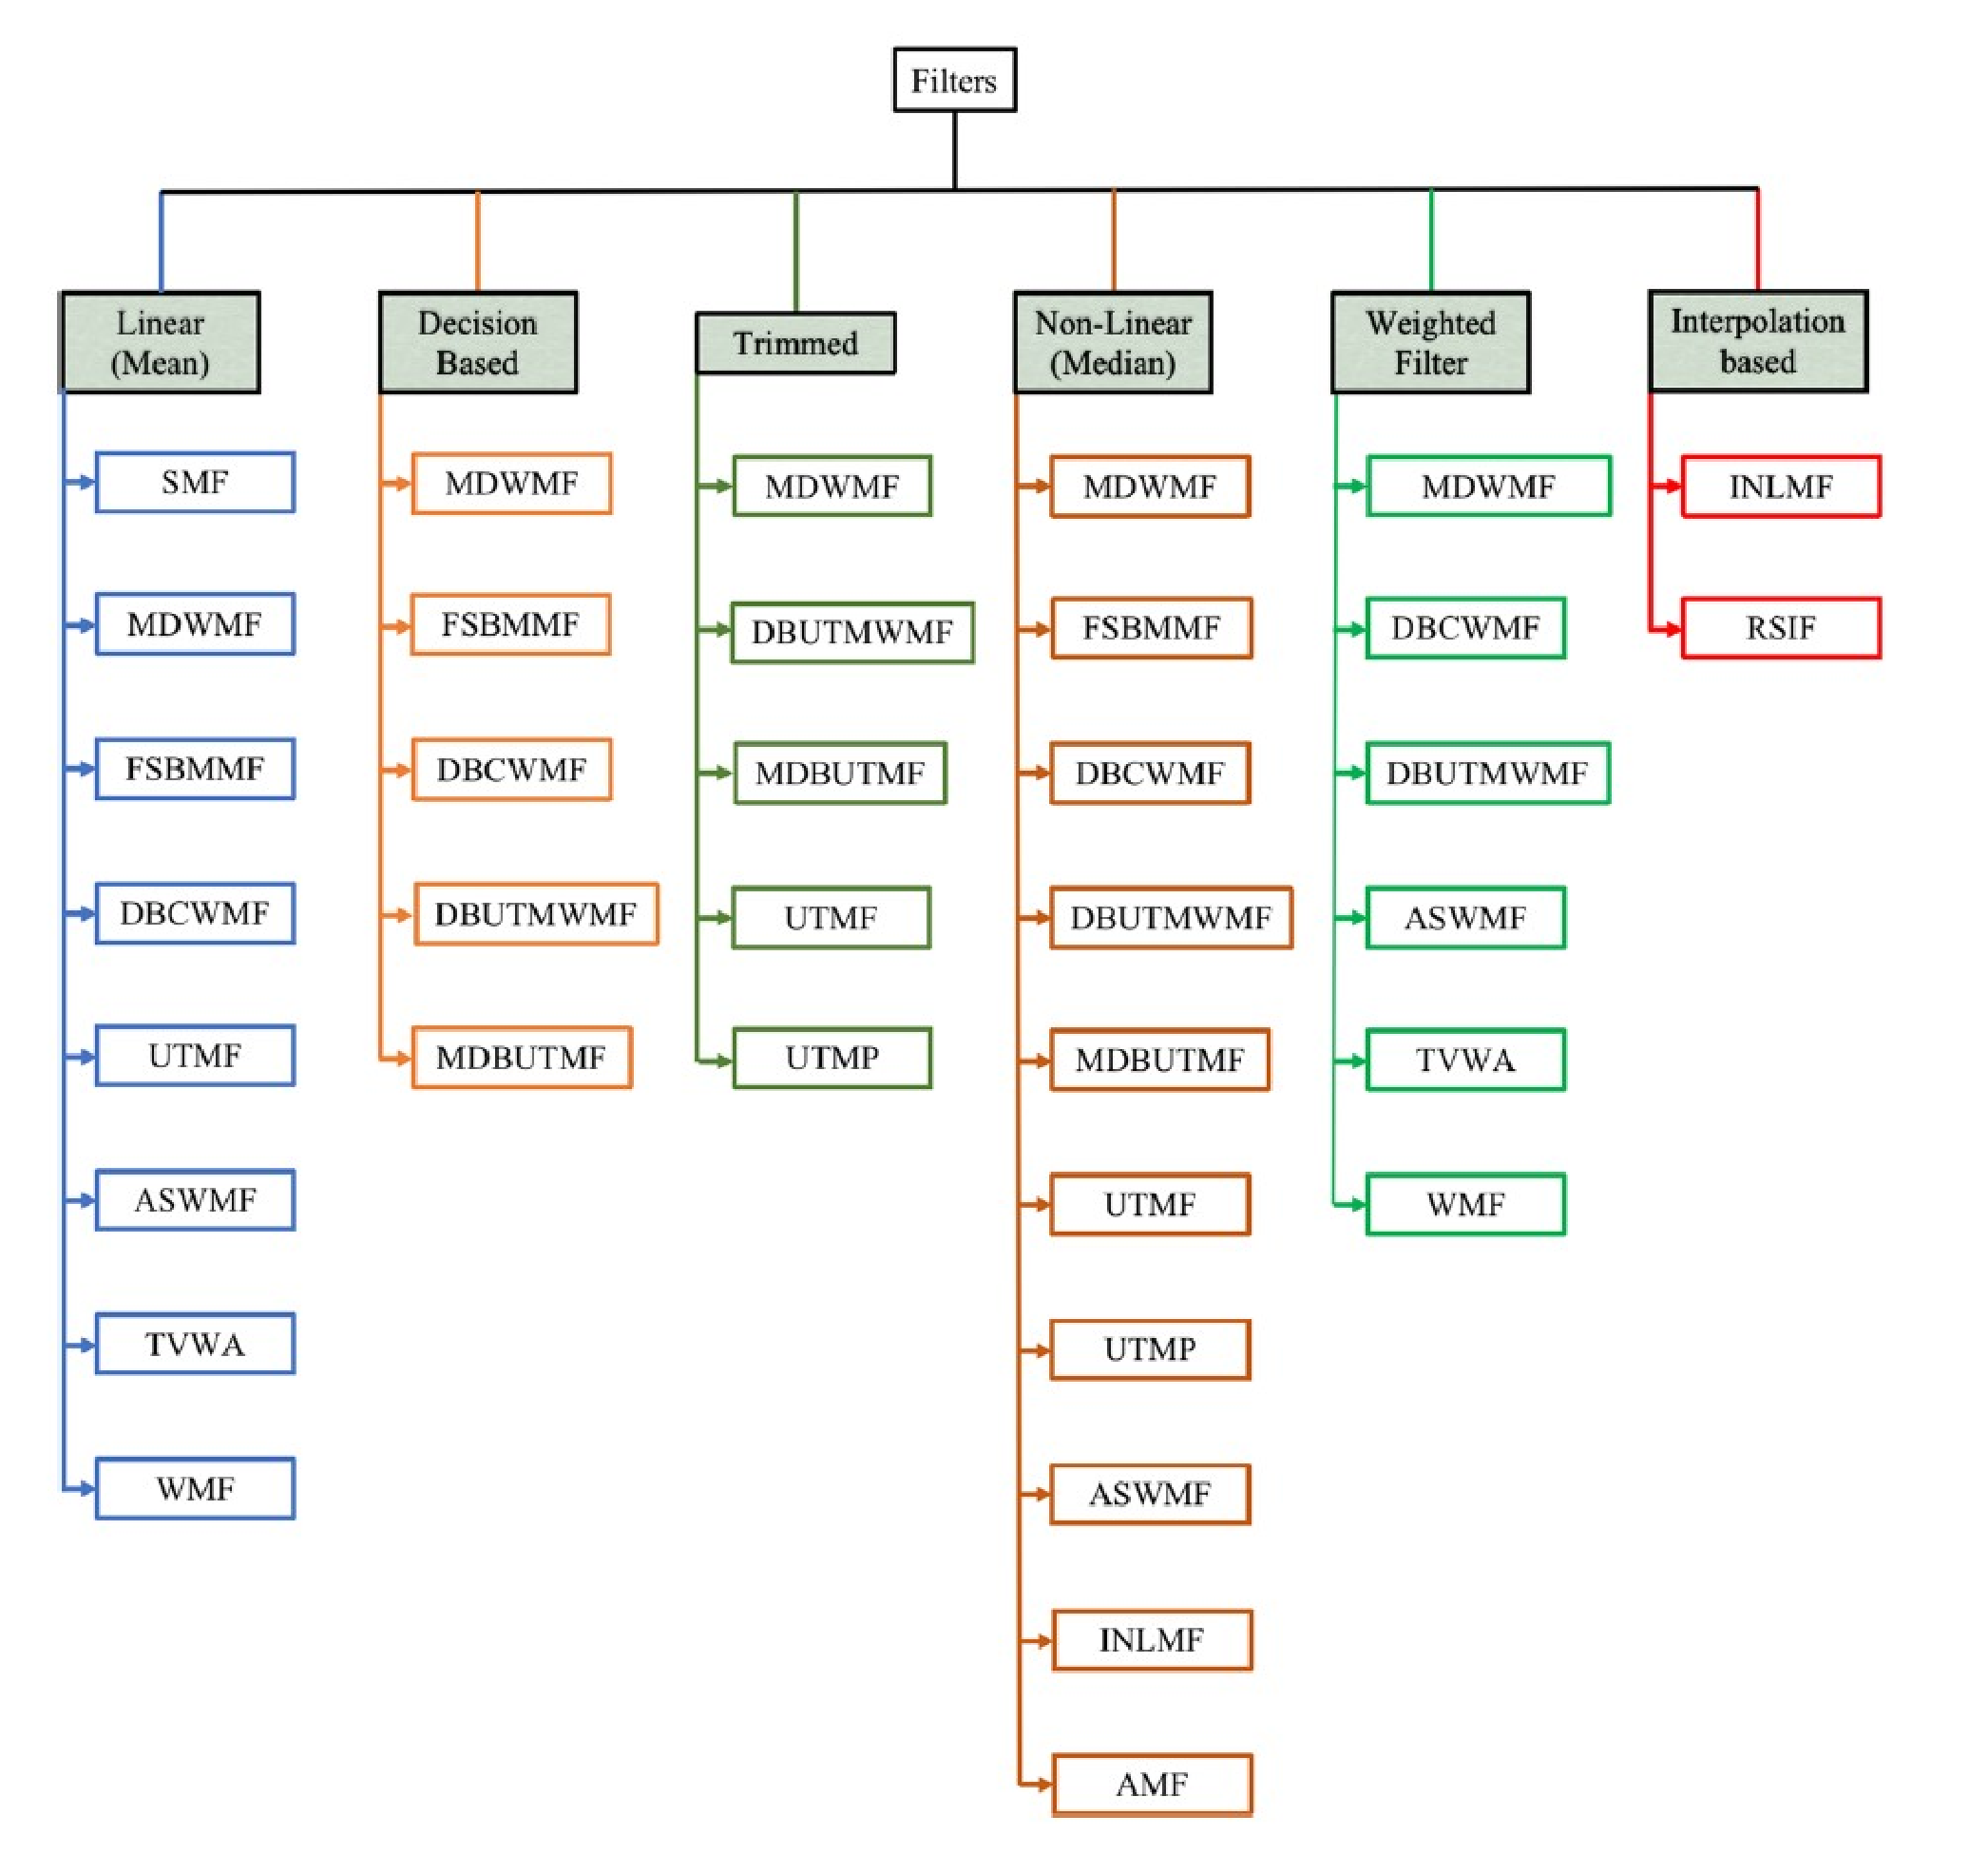
\includegraphics[width=0.6\textwidth]{images/001.eps}
    \caption{各种盐和胡椒噪声去除技术的分类流程图}
    \label{fig:meanfilter}
\end{figure}
其中,$f(x,y)$是去噪图像,$g(x,y)$是M×N维的原始图像。

\subsubsection{加权平均滤波器}
这可以看作是简单的平均滤波技术的进步。均值滤波和加权均值滤波的主要区别在于,局部邻域内的指定像素被乘以权重
矩阵中指定的权重[29, 32]。这种滤波器的数学表达式如下。

\begin{equation}
    f(x, y)=\frac{\sum_{s=-a}^a \sum_{t=-b}^b w(s, t) g(x+s, y+t)}{\sum_{s=-a}^a \sum_{t=-b}^b w(s, t)}
\end{equation}

\subsection{非线性滤波器}
一些非线性滤波器[2-4, 7, 10-12, 16, 18-20, 29, 31]被开发出来,以提供比线性滤波器更好的性能并克服其缺点。
顾名思义,这一类的滤波器不满足叠加。本节对文献中存在的各种非线性滤波器进行了全面回顾。

\subsubsection{中值滤波器}
它也可以被称为顺序统计滤波器。它是简单而最强大的非线性滤波器。像平均数滤波器一样,它也通过平滑图像来消除噪音。
它用所选窗口或内核的中值替换图像的像素值。这也降低了图像中不同像素之间的强度变化。一个给定的窗口/向量的中值的
计算方法是,首先将它们按升序排列,然后选择重新排列的窗口/向量的中间值。如果所选窗口/向量中的像素数是偶数,那么
中值是通过平均两个中间像素值来计算。以下是这个过滤器的方程式。
\begin{equation}
    f(x, y)=\operatorname{Median}[g(s, t)]
\end{equation}

其中$S_{xy}$是计算中值的区域。与线性滤波器相比,中值滤波器在消除盐和胡椒噪声方面更有效。中值滤波器比线性滤波器的主
要优点是,前者可以有效地消除输入图像中非常大的噪声影响。标准中值滤波器通常在低噪声密度下更有效。在较高的噪声下,
增加处理窗口的大小会导致输出模糊,而小窗口的噪声抑制效果不佳。

\subsubsection{切换式中值滤波器}
这是对标准中值滤波器的修改。滤波器中使用的噪声检测算法决定了损坏的像素、未损坏的像素以及校正算法如何使用中值公式
[12, 20, 29, 31]。

\subsubsection{渐进式开关中值滤波器}
这个过滤器根据预定义的固定阈值对像素的检测作出决定。主要的挑战是如何固定阈值以准确地检测出有噪声的像素。这种
滤波器在高密度下不能正确地保留边缘,因为这种滤波器在执行其操作时不考虑局部细节[12, 20, 29, 31]。

\subsubsection{截尾均值滤波器}
这个过滤器使用基于决策的算法。它首先使用3×3的窗口进行去噪。如果处理窗口没有非噪声像素,那么中心像素就被窗口
的平均值取代,否则就被窗口的中值取代[3]。

\subsubsection{非对称性截尾中值滤波器}
在这个滤波器中,对排序窗口两侧的损坏像素进行不对称的修剪。修剪后的窗口的中位数被计算出来,并取代了处理后的像素。
因此,如果产生的修剪后的窗口是空的,它将不起作用,这主要发生在高噪声密度下。因此,它在高噪声密度下不能很好地工
作,而且也不能保留边缘细节[11]。

\subsubsection{最小滤波器}
在这个滤波器中,像素值被具有最小强度水平的相邻像素的值所取代。由于其程序,它也被称为第0百分位数滤波器。这意味着
它适合图像中最暗的像素。

\subsubsection{最大滤波器}
在这个滤波器中,像素值被损坏的处理像素附近的最亮的像素所取代。它也被称为第100百分位数滤波器。它可以去除图像中的
胡椒粉噪音。

\subsection{基于决策的算法(DBA)}
在高噪声密度下,被破坏的中心像素被无噪声的邻近像素所取代。当与邻近像素重复替换时,也会出现条纹效应[3, 4, 11, 26]。

\subsubsection{改进DBA}
这个滤波器是为了避免在DBA中观察到的条纹效应。在这里,中断的中心像素的值是通过计算不对称修剪的处理窗口的中值来
计算的。然而,在高噪声密度下,该滤波器的效率很差或非常低。

\subsection{自适应滤波器}
顾名思义,这些[1, 2, 12, 16, 19, 21, 32].类型的过滤器的行为随着图像区域和过滤器区域的统计特征变化而变化。这些
过滤器很难实现,而且比其他过滤器的性能更好。这种去噪算法所涉及的步骤是:
\begin{enumerate}
    \item 分析:在这个步骤中类似的图像块被收集成组。
    \item 处理:得到的组通过阈值进行过滤。
    \item 合成:然后,过滤后的区块将用于最终的图像重建,该图像重建是由过滤后的区块上的操作计算出来的。
\end{enumerate}

\subsubsection{自适应中值滤波器}
最常用的自适应滤波器是 "自适应中值滤波器" [16]。它在过滤图像的同时保留了图像的细节。它在含有高密度盐和胡椒噪声
的图像上也表现良好。这个滤波器的一个有趣的特点是,它可以在操作过程中根据预定的条件改变其窗口大小。这个过滤器涉
及的步骤如下:
\begin{enumerate}
    \item 它会计算出受噪声影响的窗口的极端值。
    \item 检查计算出的中位数本身是否是一个极端值(即盐和胡椒的噪音)。
    \item 如果中值也是一个被破坏的值,那么就用增加的窗口大小重申这一过程,并计算中值。窗口大小可以增加到预定的最大窗口大小。否则,进入下一个步骤。
    \item 检查被处理的像素的值是否被破坏。如果被破坏,则用之前计算的中位数替换该像素,否则该像素保持不变。
\end{enumerate}
AMF在低度和中度噪声密度下工作良好。它在图像中引入了模糊效应,因为它使用的可变窗口大小有时很大,导致重建的图像
中出现模糊效应。

\subsubsection{自适应里兹平均滤波器}
作者提出了自适应里兹平均滤波(ARMF[8])。使用的主要概念是像素相似性,用于像素去噪。它在将图像转换为双重形式后
对其进行操作。它使用基于相似性的Riesz平均值。它比其他不同的相似性或距离函数(如p-norm、Euclid和Hamming)表现
得更好。它也被优化来完成所有这些操作。通过使用噪声检测掩码或另一个平均值并使用相同的像素相似度概念,也有改进的
余地。

\subsubsection{NRSMMF}
它[25]是一种独特的技术,根据图像的噪声密度选择要执行的操作。基本操作是。平均数、中位数、预处理值。在恢复被极高
密度噪声破坏的图像方面非常有效。它使用三个噪声密度范围。对于噪声密度小于等于25\%,它检查一系列的4个条件来恢复
像素值。如果噪声密度小于85\%且大于25\%,它计算5×5窗口中先前处理的像素的平均值。否则,如果噪声密度大于85\%,
则计算5×5窗口中先前处理的像素的平均值。这个过滤器根据特定窗口的信息做出准确的决定。

\subsubsection{AWM3F}
开发这个[23]算法的动机是为了过滤密度非常高的SAP噪声(即大于85\%)。该算法使用对称填充和自适应窗口大小的概念。
在第一步中,该算法试图选择有足够的非噪声像素的窗口大小进行去噪。基本操作是找到:窗口中的最小、最大和中间像素
值,并找出它们的权重。在这里,使用所选窗口的最小值和最大值来计算两组高度相关的无噪声像素。如果没有找到,其大
小将增加一个。最大尺寸可以是7×7。

\subsubsection{AFMF}
这个[9]滤波器可以被认为是自适应中值滤波器(AMF)的一个发展。它计算频率中位数而不是振幅中位数来恢复噪声像素的
像素值。这种修改产生了比AMF更好的结果,因为恢复的像素值非常接近于原始像素值。其原因可能是在频域中进行的操作。
这将在评估恢复的像素值时排除嘈杂的像素,并将重点放在恢复值的唯一性上。

\substection{组合滤波器}
这些滤波器利用线性和非线性相结合的方法来恢复噪音像素。根据噪声密度或处理窗口中无噪声像素的可用性,这些滤波器要
么使用线性方法,如均值、插值等,要么使用非线性技术,如中值进行去噪。以下各小节讨论了最近提出的各种组合滤波器。

\subsubsection{基于模态决策的非对称修剪中值(MDBUTM)滤波器}
在这个滤波器中,计算处理窗口中非噪声像素的中值,用计算出的中值替换损坏的处理像素[11]。此外,如果一个窗口中的
所有像素值都被破坏了,那么就计算处理窗口的平均值来替换中央被破坏的像素。然而,这种方法会导致过滤器的性能变差,
因为这相当于给损坏的像素分配任何随机值,而不是'0'或'255'值。
\end{document}
